\documentclass[11pt,a4paper]{article}

\usepackage[T1]{fontenc}
\usepackage[utf8]{inputenc}
\usepackage[french]{babel}
\usepackage{lmodern}
\usepackage{amsmath,amssymb}
\usepackage[locale=FR]{siunitx}
\usepackage{booktabs}
\usepackage{graphicx}
\usepackage{float}
\usepackage[margin=2.2cm]{geometry}
\usepackage{xcolor}
\usepackage{enumitem}
\usepackage{caption}
\usepackage[colorlinks=true,linkcolor=blue!50!black,urlcolor=blue!50!black,citecolor=blue!50!black]{hyperref}

\graphicspath{{./}{../cases/}{../echantillon/}}
\captionsetup{font=small,labelfont=bf}

\newcommand{\code}[1]{\texttt{#1}}
\newcommand{\Kcell}{K_{\mathrm{cell}}}

\title{Étude paramétrique $(\xi,\zeta)$ sur des échantillons de type \emph{Frank}\\[3pt]
  \large Compte rendu de la campagne \code{etude-param-frank}}
\author{\textsc{l-hyphen}}
\date{\today}

\begin{document}
\maketitle

\begin{abstract}
  On étudie l'influence de deux rapports de raideurs sans dimension, $\xi$ (flexion des parois / traction des
  parois) et $\zeta$ (cohésion entre cellules / raideur d'une cellule), sur la réponse d'un échantillon entaillé de
  cellules molles soumis à une ouverture imposée. La campagne compte 121 simulations
  ($\xi,\zeta\in\{0.1,\,0.25,\,0.5,\,0.75,\,1,\,2,\,3,\,4,\,5,\,7.5,\,10\}$) sur un échantillon de mêmes
  dimensions et de même nombre de cellules que celui de \emph{Frank-ouverture-fissure}. La raideur apparente suit
  très précisément un modèle de deux ressorts en série (cellules et liens cohésifs) ; la force au pic croît
  comme $\zeta^{1/4}$ à $\zeta^{1/3}$ et passe par un maximum en $\xi$ lorsque la cohésion est forte ; la
  fissure principale, isolée de ses ramifications par \code{crackwatch}, se propage à une vitesse de 0.55 à 0.8
  fois une vitesse d'onde élastique de l'échantillon, et devient tortueuse et ramifiée pour $\zeta\gtrsim 2$.
\end{abstract}

\tableofcontents

%======================================================================
\section{Paramètres étudiés}
%======================================================================

Chaque cellule est un polygone de nœuds reliés par des barres. Une barre de longueur moyenne $\ell$ a une raideur
axiale $k_s$ (N/m) ; deux barres consécutives ont une raideur de flexion $k_b$ (N·m/rad) ; deux cellules voisines
sont reliées par des liens cohésifs de raideur $k_c$ (N/m), qui servent aussi de raideur de contact
($k_n=k_t=k_c$). On définit
\begin{equation}
  \xi = \frac{k_b}{k_s\,\ell^2},\qquad
  \Kcell = \frac{12\,\xi\,k_s}{1+9\,\xi},\qquad
  \zeta = \frac{k_c}{\Kcell}.
\end{equation}
$\xi$ compare la raideur de flexion des parois à leur raideur axiale ; $\Kcell$ est la raideur d'une cellule,
qui combine ces deux mécanismes (elle tend vers $\tfrac{4}{3}k_s$ quand $\xi\to\infty$ et vers $12\,\xi\,k_s$
quand $\xi\to 0$) ; $\zeta$ compare la raideur de la cohésion à celle des cellules. À $k_s$ fixé, on en déduit
\begin{equation}
  k_b = \xi\,k_s\,\ell^2,\qquad k_c = \zeta\,\Kcell .
\end{equation}

La cohésion suit un modèle en énergie : une face collée de longueur $L$ stocke dans ses points de colle une
énergie élastique $W$, et rompt lorsque le taux de restitution $G=W/(2L)$ atteint $G_c$. Ce modèle est
élastique-fragile : il n'y a pas d'adoucissement.

\begin{table}[H]
  \centering
  \small\begin{tabular}{lll}
    \toprule
    Grandeur & Valeur & Remarque \\
    \midrule
    $k_s$ & \SI{2000}{N/m} & valeur de \emph{Frank-ouverture-fissure} \\
    $\ell$ & \SI{1.986e-4}{m} & longueur moyenne des barres de l'échantillon \\
    $G_c$ & \SI{1.2575e-6}{J/m} & énergie de rupture des liens \\
    masse des nœuds & \SI{8e-8}{kg} & \\
    largeur des parois (\code{barWidth}) & \SI{2e-6}{m} & \\
    $\Delta t$ & \SI{5e-8}{s} & $\Delta t_{\mathrm{crit}}/\Delta t\geq 16$ sur toute la grille \\
    vitesse des mors & $\pm$\SI{0.3}{mm/s} & ouverture à \SI{0.6}{mm/s} \\
    \bottomrule
  \end{tabular}
  \caption{Grandeurs fixes de la campagne. Pour $\xi=\zeta=10$, on retrouve les raideurs de
    \emph{Frank-ouverture-fissure} (à $\ell$ près).}
\end{table}

%======================================================================
\section{Campagne}
%======================================================================

\paragraph{Échantillon.} Un unique pavage, généré par \code{nodegen}, sert à tous les cas
(figure~\ref{fig:echantillon}) : \SI{13.6}{mm} $\times$ \SI{16}{mm}, 2222 cellules (13\,084 nœuds) de diamètre
équivalent \SI{0.353}{mm}, réseau hexagonal perturbé (88\,\% d'hexagones), aucune barre courte
($\ell_{\min}/\bar\ell = 0.40$). Une pré-entaille nette de \SI{1.2}{mm} part du milieu du bord gauche ; sa pointe
effective est en $(1.181,\,8)$~mm, à \SI{12.42}{mm} du bord droit (ligament). Les mors pilotent la rangée de nœuds
du bord haut (79 nœuds) et du bord bas (82 nœuds).

\begin{figure}[H]
  \centering
  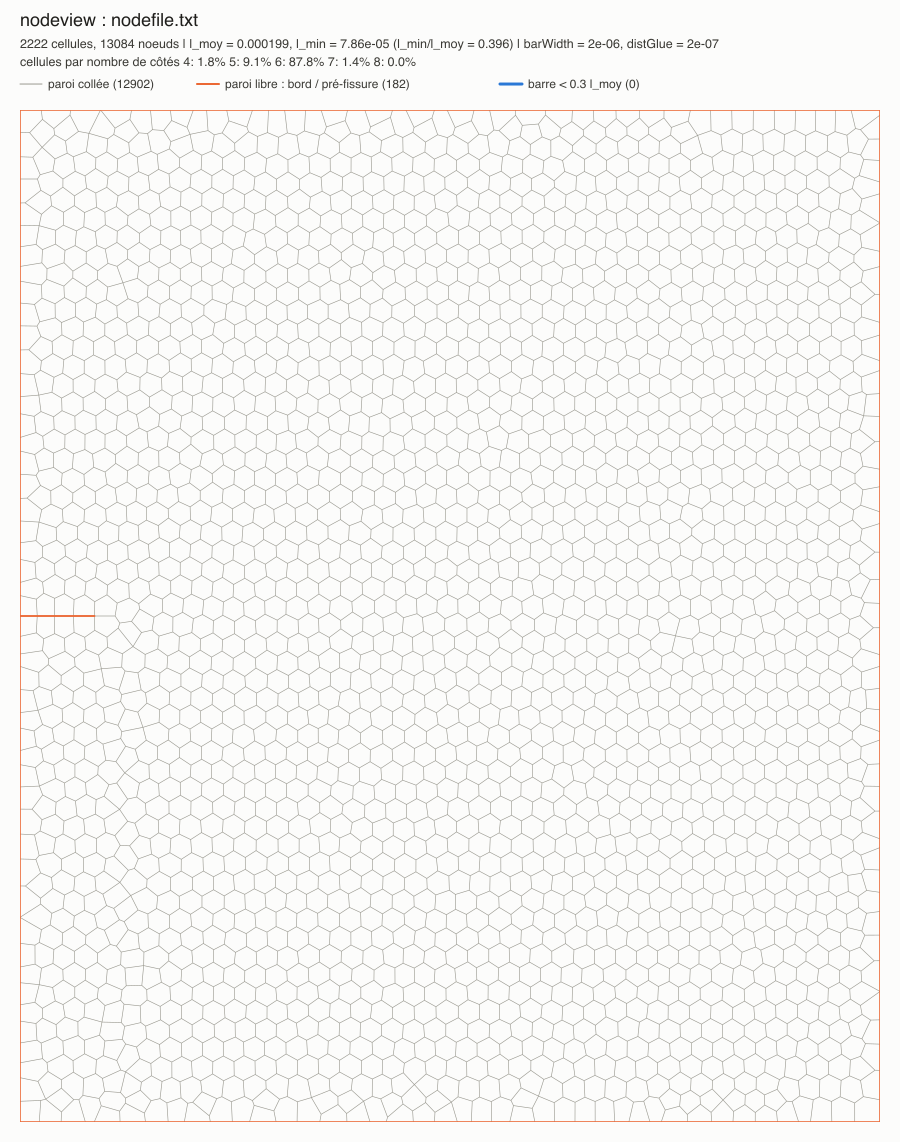
\includegraphics[width=0.55\textwidth]{echantillon.png}
  \caption{Échantillon commun aux 121 cas.}
  \label{fig:echantillon}
\end{figure}

\paragraph{Plan.} Toutes les combinaisons de
$\xi,\zeta\in\{0.1,\,0.25,\,0.5,\,0.75,\,1,\,2,\,3,\,4,\,5,\,7.5,\,10\}$, soit $11\times 11=121$ cas. Le
générateur \code{generate\_cases} écrit, à partir d'un même modèle d'input, un répertoire par cas dans lequel seules
les lignes \code{define XI} et \code{define ZETA} changent ; $k_b$ et $k_c$ sont calculés par \textsc{l-hyphen}.

\paragraph{Arrêt et sorties.} Chaque calcul s'arrête \SI{5}{ms} après une chute de 30\,\% de la force du mors
haut (événement \code{stopAfterStressDrop}), ce qui laisse à la fissure le temps de traverser l'échantillon. Les
forces des mors sont écrites toutes les \SI{0.1}{ms} (\code{nstepPeriodCapture}), les configurations toutes les
\SI{1}{ms}, plus une configuration à la première rupture de lien ; \code{breakHistory.txt} enregistre chaque
rupture (instant, faces, énergie libérée).

\paragraph{Coût.} Les 121 cas se sont terminés par l'événement d'arrêt, sans échec, entre \SI{27}{ms} et
\SI{65}{ms} de temps simulé. Il a fallu \SI{13}{min} de calcul par cas en moyenne (\SI{10}{} à \SI{24}{min}), avec
4 calculs simultanés, et \SI{15}{Go} de disque au total.

\paragraph{Dépouillement.} Les figures sont produites par les scripts de \code{cases/} : \code{plot\_maps.py}
(raideur et forces), \code{plot\_curves.py} (courbes force--ouverture), \code{plot\_breaks.py}
(\code{breakHistory.txt} et \code{breakEvol.txt}), \code{plot\_crackwatch.py} (fissure principale et
ramifications), \code{plot\_snapshots.py} (rendus \code{see2}) ; deux figures propres à ce document viennent de
\code{rapport/figures\_rapport.py}. Dans toutes les cartes, $\xi$ croît de gauche à droite et $\zeta$ de bas en
haut ; les courbes « en fonction de chaque paramètre » tracent une grandeur en fonction de $\xi$ (une courbe par
$\zeta$) et de $\zeta$ (une courbe par $\xi$), la couleur suivant la valeur du paramètre fixé.

\paragraph{Une seule réalisation.} Chaque couple $(\xi,\zeta)$ n'est simulé qu'une fois, sur le même pavage.
Les grandeurs qui dépendent du chemin de la fissure (ramifications, longueur rompue) varient donc fortement d'un
cas à son voisin ; il faut les lire comme des tendances. Les grandeurs globales (raideur, force au pic, vitesse
de la fissure principale) sont, elles, très régulières.

%======================================================================
\section{Réponse globale}
%======================================================================

\subsection{Courbes force--ouverture}

La force est la moyenne des réactions des deux mors, l'ouverture la variation de distance entre eux
(figure~\ref{fig:courbes}, mêmes axes pour tous les cas). Toutes les réponses sont linéaires jusqu'au pic puis
chutent brutalement : la rupture est fragile, comme le veut le modèle de cohésion. Le premier lien rompt à 93\,\%
au moins de la force au pic, et presque toujours au pic lui-même ; la fissure n'a pas de phase de propagation
stable. Après la chute, la force présente des rebonds qui reviennent à zéro : ce sont des oscillations dynamiques
des deux moitiés séparées, le calcul étant sans dissipation globale ; ils ne sont pas exploités.

Exception notable : pour $\xi=2$ et $3$ avec $\zeta\geq 5$, le pic (point plein) est distinct du premier lien rompu
(point creux). La fissure s'amorce, s'arrête après quelques liens, puis repart plus tard sous une force un peu plus
élevée (section~\ref{sec:principale}).

\begin{figure}[p]
  \centering
  \includegraphics[width=\textwidth]{courbes_force_ouverture.png}
  \caption{Courbes force--ouverture des 121 cas (ouverture 0--\SI{38.9}{\micro m}, force 0--\SI{59.3}{mN}).
    Point creux : premier lien rompu ; point plein : pic, lorsqu'il en diffère.}
  \label{fig:courbes}
\end{figure}

\subsection{Raideur}

La raideur $K$ est la pente de la courbe force--ouverture, ajustée sous 50\,\% du pic
(figure~\ref{fig:raideur}). Elle croît avec $\xi$ et avec $\zeta$ et sature dans les deux directions, de
\SI{282}{N/m} ($\xi=\zeta=0.1$) à \SI{2540}{N/m} ($\xi=\zeta=10$).

\begin{figure}[p]
  \centering
  \includegraphics[width=0.62\textwidth]{carte_raideur.png}\\[4pt]
  \includegraphics[width=\textwidth]{courbes_parametres.png}
  \caption{Raideur, force au pic et force maximale avant la première rupture. En haut : carte de la raideur. En
    bas : chaque grandeur en fonction de $\xi$ et de $\zeta$ ; le point creux en 0 est la limite sans cohésion
    ($k_c=0$), non simulée.}
  \label{fig:raideur}
\end{figure}

Cette dépendance s'explique entièrement par deux ressorts en série, les cellules ($\Kcell$) et les liens cohésifs
($k_c=\zeta\Kcell$). L'ajustement des 121 raideurs sur
\begin{equation}
  \frac{1}{K} = \frac{a}{\Kcell} + \frac{b}{k_c}
  \quad\Longleftrightarrow\quad
  \frac{K}{\Kcell} = \frac{\zeta}{a\,\zeta + b}
\end{equation}
donne $a=1.003$ et $b=0.350$, avec un écart de 1\,\% en médiane et 4\,\% au plus
(figure~\ref{fig:serie}). Toutes les courbes se superposent une fois $K$ rapportée à $\Kcell$ : $\xi$ n'agit sur la
raideur qu'à travers $\Kcell$. Le coefficient $a\simeq 1$ signifie que, pour cet échantillon, la raideur du réseau
de cellules sans liens souples vaut $\Kcell$ ; $b=0.35$ mesure le poids relatif des interfaces : la cohésion
divise la raideur par deux pour $\zeta\approx 0.35$ et ne lui retire plus que 4\,\% pour $\zeta=10$. Les petits
écarts au modèle concernent $\xi=0.1$ aux grands $\zeta$ (points clairs au-dessus de la courbe).

\begin{figure}[H]
  \centering
  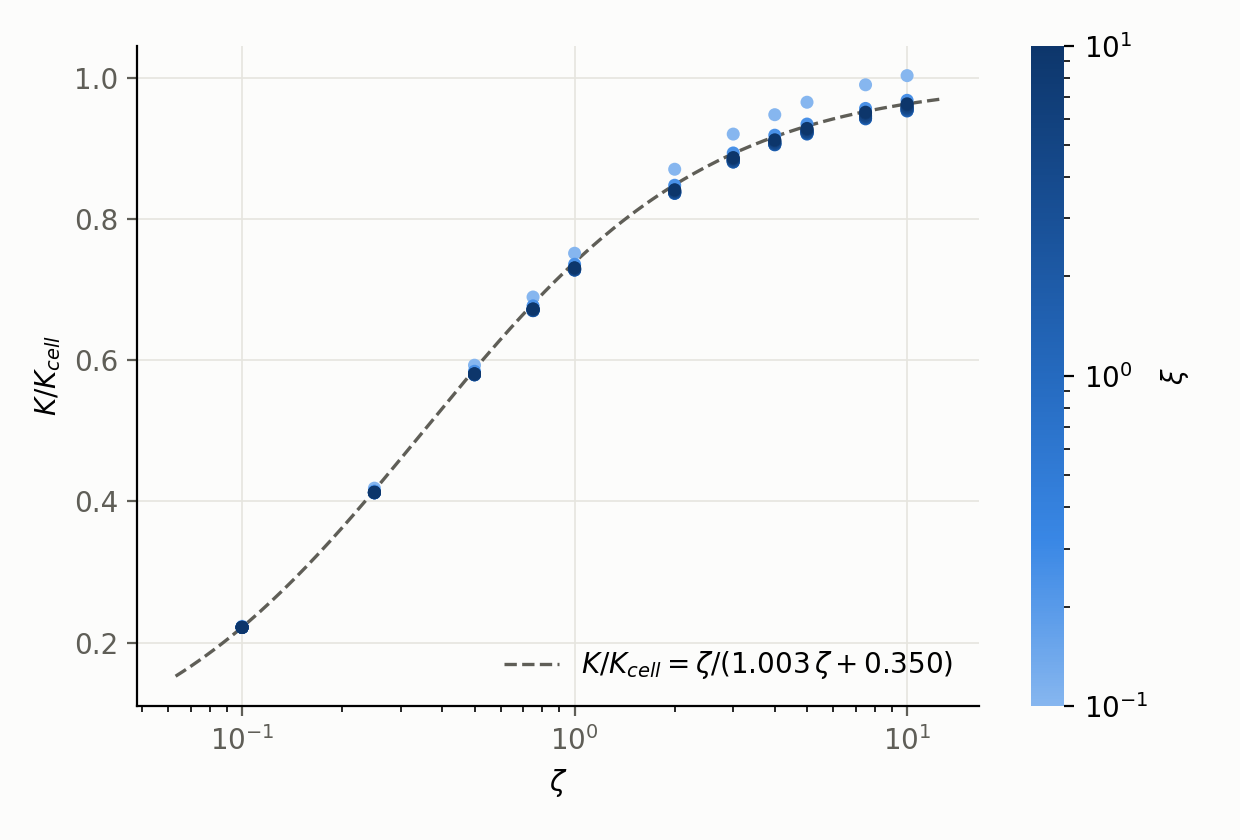
\includegraphics[width=0.62\textwidth]{fig_raideur_serie.png}
  \caption{Raideur rapportée à $\Kcell$ : les 121 cas suivent le modèle de deux ressorts en série (tirets).}
  \label{fig:serie}
\end{figure}

\subsection{Force à la rupture}

La force au pic (figure~\ref{fig:forces}) va de \SI{8.4}{mN} à \SI{53.9}{mN}. Elle croît avec $\zeta$ comme une
puissance faible : $F_{\mathrm{pic}}\propto\zeta^{0.36}$ pour $\xi=0.1$, $\zeta^{0.32}$ pour $\xi=1$ et
$\zeta^{0.25}$ pour $\xi=10$. Pour $\zeta\leq 1$, elle croît aussi avec $\xi$ et sature dès $\xi\approx 1$. Pour
$\zeta\geq 2$, elle passe par un maximum en $\xi$ ($\xi=1$ pour $\zeta=2$, $0.75$ pour $\zeta=3$, $0.5$ pour
$\zeta\geq 4$), puis décroît : à $\zeta=10$, elle perd 21\,\% entre $\xi=0.5$ (\SI{53.9}{mN}) et $\xi=10$
(\SI{42.6}{mN}). La force maximale avant la première rupture suit les mêmes tendances, avec une décroissance en
$\xi$ plus marquée, parce que les cas $\xi=2$--$3$ s'amorcent avant leur pic.

Une interprétation possible, à vérifier, de cette décroissance : lorsque les parois sont raides en flexion, les
cellules en pointe d'entaille se déforment moins, émoussent moins la concentration de contrainte et transmettent
une charge plus localisée aux premiers liens.

L'ouverture au pic est minimale vers $\zeta\approx 0.75$--1 (\SI{12.6}{\micro m} à \SI{19}{\micro m}) et
croît de part et d'autre (jusqu'à \SI{35}{\micro m}) : aux faibles $\zeta$ la raideur est petite, aux forts
$\zeta$ la force continue de croître alors que la raideur sature. L'instant de la première rupture suit
l'ouverture au pic : l'ouverture croît à \SI{0.605}{\micro m/ms}, soit la vitesse imposée.

\begin{figure}[H]
  \centering
  \includegraphics[width=\textwidth]{carte_forces_rupture.png}
  \caption{Force au pic et force maximale avant la première rupture de lien (même échelle de couleur).}
  \label{fig:forces}
\end{figure}

%======================================================================
\section{Faciès et quantité de rupture}
%======================================================================

\subsection{Faciès}

La figure~\ref{fig:faciesbrut} montre les liens rompus dans le dernier conf de chaque cas. Pour $\zeta\leq 0.25$,
la fissure est droite et traverse l'échantillon le long de la ligne de l'entaille, avec très peu de branches. Pour
$\zeta$ entre 0.5 et 1, de courtes branches apparaissent mais s'arrêtent vite. À partir de $\zeta=2$, la
fissure dévie, se dédouble (souvent en Y, deux branches presque symétriques vers le bord droit pour
$\xi=2$--$4$) ou part en biais. La colonne $\xi=0.1$ fait exception : la fissure y reste droite pour tous
les $\zeta$.

\begin{figure}[p]
  \centering
  \includegraphics[width=\textwidth]{images_rupture.png}
  \caption{Faciès de rupture (\code{see2}, dernier conf, liens rompus en rouge).}
  \label{fig:faciesbrut}
\end{figure}

\subsection{Longueur rompue et énergie libérée}

La figure~\ref{fig:ruptures} donne, à partir de \code{breakHistory.txt} et \code{breakEvol.txt}, la longueur
rompue rapportée au ligament (\SI{12.42}{mm}), l'énergie libérée, la durée et la vitesse moyenne de propagation.
La longueur rompue va de 1.16 fois le ligament (fissure droite, $\zeta=0.1$) à 2.2 fois (fissures ramifiées,
$\zeta=2$--$4$).

L'énergie libérée n'apporte pas d'information supplémentaire : avec le modèle de cohésion, chaque face rompt
exactement quand $W=2\,G_c\,L$, et l'énergie libérée totale vaut $2\,G_c$ fois la longueur rompue (le rapport des
deux est compris entre 1.000 et 1.005 sur les 121 cas). La carte d'énergie est donc la carte de longueur
rompue à une constante près.

La durée et la vitesse moyenne de propagation sont bruitées : elles mélangent la fissure principale et ses
ramifications, et incluent les arrêts de la fissure. La figure~\ref{fig:longueur} montre ces arrêts : pour
$\xi=2$--$3$ et $\zeta\geq 5$, la longueur rompue reste bloquée pendant 2 à \SI{3}{ms} après les premières
ruptures. Ces mesures globales sont remplacées dans la section suivante par celles de la seule fissure principale.

\begin{figure}[p]
  \centering
  \includegraphics[width=\textwidth]{carte_ruptures.png}
  \caption{Longueur rompue / ligament, énergie libérée, durée de propagation (1re rupture à 90\,\% de la longueur
    finale) et vitesse moyenne ($0.9\times$ longueur finale / durée).}
  \label{fig:ruptures}
\end{figure}

\begin{figure}[p]
  \centering
  \includegraphics[width=\textwidth]{courbes_longueur_rompue.png}
  \caption{Longueur rompue cumulée (toutes fissures) en fonction du temps depuis la première rupture. Pointillés :
    fissure droite à travers le ligament.}
  \label{fig:longueur}
\end{figure}

\begin{figure}[p]
  \centering
  \includegraphics[width=\textwidth]{courbes_parametres_ruptures.png}
  \caption{Grandeurs de la figure~\ref{fig:ruptures} en fonction de chaque paramètre.}
  \label{fig:courbesruptures}
\end{figure}

%======================================================================
\section{Fissure principale et ramifications}
\label{sec:principale}
%======================================================================

\subsection{Méthode}

\code{crackwatch} construit le graphe des faces rompues à partir de \code{breakHistory.txt} et des positions
initiales (\code{conf0}). Il fusionne les nœuds proches et découpe le graphe en fissures (composantes connexes).
Son propre « chemin principal », le plus long des plus courts chemins entre deux extrémités, peut relier deux
pointes de ramifications sans passer par l'entaille (c'est le cas pour $\xi=3$, $\zeta=2$ et 4). On définit donc la
\textbf{fissure principale} comme le plus court chemin dans le graphe entre la pointe de l'entaille et
l'extrémité de la même fissure la plus éloignée de cette pointe. Le reste des liens rompus forme les ramifications
et les fissures secondaires. On mesure ensuite :
\begin{itemize}[nosep]
  \item la \textbf{tortuosité} : longueur de la fissure principale / distance entre ses extrémités ;
  \item la \textbf{part des ramifications} : $1-$ longueur de la fissure principale / longueur rompue totale ;
  \item la \textbf{vitesse} de la fissure principale : pente de sa longueur rompue en fonction du temps, ajustée
    entre 20\,\% et 60\,\% de sa longueur finale (au-delà, certaines fissures s'arrêtent avant le bord) ;
  \item le \textbf{délai d'amorçage} : de la première rupture à 20\,\% de la longueur de la fissure principale.
\end{itemize}

La figure~\ref{fig:faciescw} montre le résultat : fissure principale en bleu foncé, ramifications en orange.
Une seule fissure par cas, sauf pour $\xi=0.1$ avec $\zeta\geq 5$, où de petites fissures secondaires
apparaissent près du mors bas.

\begin{figure}[p]
  \centering
  \includegraphics[width=\textwidth]{facies_crackwatch.png}
  \caption{Fissure principale (depuis la pointe de l'entaille) et ramifications, configuration initiale. Largeur
    complète de l'échantillon, hauteur limitée à la bande fissurée.}
  \label{fig:faciescw}
\end{figure}

\subsection{Résultats}

Les cartes (figure~\ref{fig:cartecw}) et les courbes (figure~\ref{fig:courbescw}) appellent les remarques
suivantes.

\paragraph{Vitesse.} Une fois les ramifications et les arrêts écartés, la vitesse de la fissure principale est la
grandeur la plus régulière de l'étude. Elle croît de façon quasi monotone avec $\xi$ et avec $\zeta$, de
\SI{4.8}{m/s} ($\xi=\zeta=0.1$) à \SI{19.8}{m/s}, avec une légère saturation en $\xi$ au-delà de 2. Les courbes
de longueur de la fissure principale (figure~\ref{fig:courbesprincipale}) sont des droites entre l'amorçage et
l'arrivée au bord, ce qui justifie une vitesse unique par cas.

Pour situer ces vitesses, on les rapporte à une vitesse d'onde élastique de l'échantillon,
$c_0=\sqrt{E_{2D}/\rho_{2D}}$, avec le module surfacique $E_{2D}=K\,H/W$ déduit de la raideur mesurée
($H=\SI{16}{mm}$, $W=\SI{13.6}{mm}$) et la masse surfacique $\rho_{2D}=\SI{4.81}{kg/m^2}$ (13\,084 nœuds de
\SI{8e-8}{kg}). $c_0$ varie de \SI{8.3}{m/s} à \SI{24.9}{m/s}. La figure~\ref{fig:onde} montre que
$v/c_0\approx 0.6$ (0.54 à 0.65) pour $\zeta\leq 1$, quel que soit $\xi$ : dans ce domaine, la vitesse de la fissure
suit la vitesse des ondes. Pour $\zeta\geq 2$, $v/c_0$ augmente avec $\xi$ et atteint 0.7 à 0.8. Ce $c_0$ n'est
qu'une échelle (il ignore l'effet de Poisson et l'anisotropie du réseau), mais ces valeurs sont du même ordre que
celles des fissures dynamiques dans les matériaux fragiles, où la vitesse limite est la vitesse de Rayleigh.

\paragraph{Tortuosité et ramifications.} La tortuosité vaut 1.15 pour les fissures les plus droites (c'est
le zigzag imposé par les parois des cellules) et monte jusqu'à 1.46. Elle reste inférieure à 1.22 pour
$\zeta\leq 1$, et vaut le plus souvent 1.25 à 1.46 pour $\zeta\geq 2$ et $\xi\geq 0.5$. La part des ramifications suit la même
transition : médiane 0.12 pour $\zeta\leq 1$, 0.25 pour $\zeta\geq 2$, quasi nulle pour $\zeta=0.1$. Elle est en
revanche très dispersée d'un cas à son voisin (de 0.04 à 0.40 aux forts $\zeta$) : le nombre et la longueur des
branches dépendent du détail du pavage, et une seule réalisation par couple ne suffit pas à les caractériser. On
n'observe pas de seuil net de vitesse au-delà duquel la fissure se ramifie (figure~\ref{fig:onde}, à droite) :
la ramification apparaît dès $v/c_0\approx 0.57$, mais des fissures plus rapides ($v/c_0>0.75$) peuvent rester
peu ramifiées.

\paragraph{Délai d'amorçage.} Il vaut 0.23 à \SI{1.23}{ms} et décroît globalement quand $\xi$ et $\zeta$
augmentent. Les cinq valeurs de 1.9 à \SI{3.2}{ms} ($\xi=2$ avec $\zeta=5$, $7.5$, $10$ ; $\xi=3$ avec
$\zeta=7.5$, $10$) sont réelles : la fissure s'arrête après les premières ruptures en pointe d'entaille, puis repart.

\begin{figure}[p]
  \centering
  \includegraphics[width=\textwidth]{carte_crackwatch.png}
  \caption{Tortuosité et vitesse de la fissure principale, part des ramifications, délai d'amorçage.}
  \label{fig:cartecw}
\end{figure}

\begin{figure}[p]
  \centering
  \includegraphics[width=\textwidth]{courbes_parametres_crackwatch.png}
  \caption{Grandeurs de la figure~\ref{fig:cartecw} en fonction de chaque paramètre.}
  \label{fig:courbescw}
\end{figure}

\begin{figure}[p]
  \centering
  \includegraphics[width=\textwidth]{courbes_fissure_principale.png}
  \caption{Longueur de la fissure principale (sans ramifications) en fonction du temps depuis la première
    rupture.}
  \label{fig:courbesprincipale}
\end{figure}

\begin{figure}[H]
  \centering
  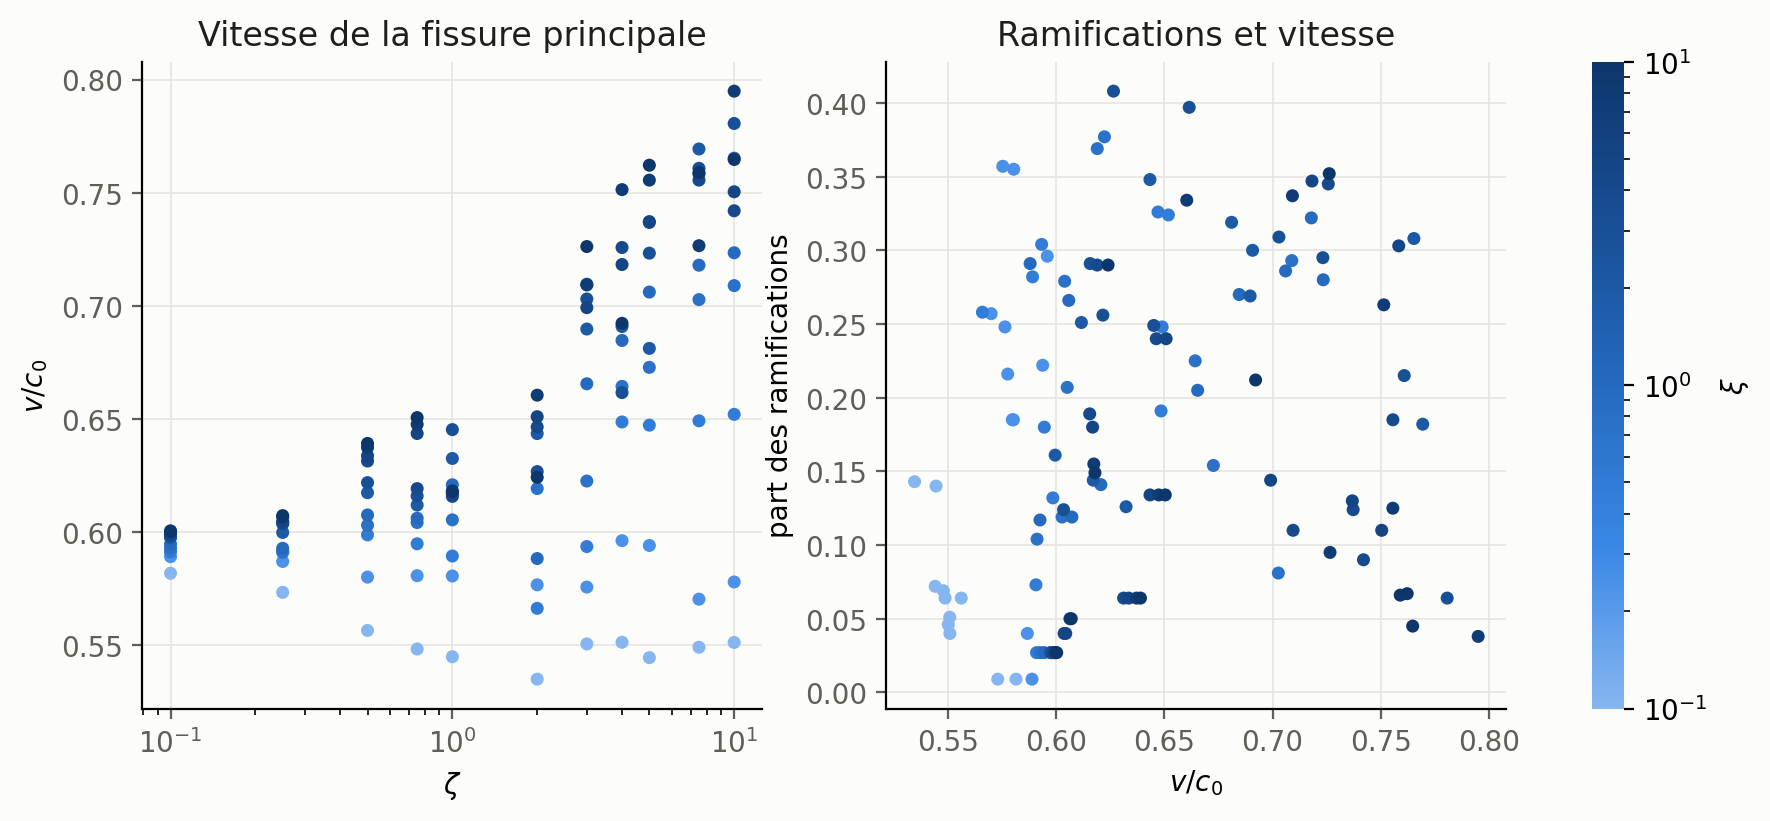
\includegraphics[width=\textwidth]{fig_vitesse_onde.png}
  \caption{À gauche : vitesse de la fissure principale rapportée à $c_0=\sqrt{E_{2D}/\rho_{2D}}$. À droite :
    part des ramifications en fonction de $v/c_0$. Couleur : $\xi$.}
  \label{fig:onde}
\end{figure}

%======================================================================
\section{Champs mécaniques}
%======================================================================

La figure~\ref{fig:contrainte} montre la contrainte $\sigma_{yy}$ au dernier conf enregistré avant le pic (échelle
commune). Les conf étant écrits toutes les millisecondes, ce conf peut précéder le pic de près d'\SI{1}{ms}. Le
champ est uniforme loin de l'entaille, avec une concentration en pointe et une zone déchargée au-dessus et
au-dessous de l'entaille ; son niveau croît avec $\zeta$, comme la force au pic. Pour $\xi=3$, $\zeta=7.5$, ce
conf tombe après les premières ruptures (amorçage puis arrêt) : une zone déchargée plus étendue entoure la pointe.

Les champs de déformation et les directions principales (déformation et contrainte, au conf de la première
rupture) sont donnés en annexe. À l'échelle de la grille complète, les directions principales sont difficiles à
lire : la traction majeure est verticale partout, sauf près de la pointe de l'entaille.

\begin{figure}[p]
  \centering
  \includegraphics[width=\textwidth]{images_contrainte.png}
  \caption{Contrainte $\sigma_{yy}$ au dernier conf avant le pic de force (échelle commune).}
  \label{fig:contrainte}
\end{figure}

%======================================================================
\section{Synthèse et perspectives}
%======================================================================

\begin{enumerate}[nosep]
  \item La raideur de l'échantillon est celle de deux ressorts en série,
    $K=\Kcell\,\zeta/(\zeta+0.35)$, à 4\,\% près sur toute la grille.
  \item La rupture est fragile dans tous les cas : la force chute dès la première rupture de lien, sauf pour
    $\xi=2$--$3$ et $\zeta\geq 5$, où la fissure s'arrête puis repart.
  \item La force au pic croît comme $\zeta^{0.25\text{--}0.36}$ ; aux forts $\zeta$, elle est maximale pour
    $\xi\approx 0.5$--$1$ et diminue de 20\,\% au-delà.
  \item Deux régimes de fissuration : pour $\zeta\leq 1$, une fissure quasi droite, peu ramifiée, à
    $v\approx 0.6\,c_0$ ; pour $\zeta\geq 2$ (et $\xi\geq 0.25$), une fissure déviée, ramifiée, plus rapide
    ($v/c_0$ jusqu'à 0.8).
  \item L'énergie libérée vaut exactement $2\,G_c$ fois la longueur rompue : elle ne mesure que la quantité de
    fissuration.
\end{enumerate}

\paragraph{Perspectives.}
\begin{itemize}[nosep]
  \item Plusieurs réalisations du pavage (graines différentes de \code{nodegen}) par couple $(\xi,\zeta)$, sur
    une grille plus grossière, pour donner une moyenne et un écart-type des grandeurs liées au chemin de la
    fissure (part des ramifications, tortuosité, arrêts).
  \item Une énergie de fracture globale tirée de l'aire sous la courbe force--ouverture, à comparer à
    $2\,G_c\times$ longueur rompue (part de l'énergie dissipée hors des liens : vibrations, contact).
  \item Une vitesse d'onde mieux définie (vitesse de Rayleigh du réseau, mesurée par exemple par le temps de
    traversée d'une impulsion) pour confirmer la comparaison $v/c_0$.
  \item Des conf plus fréquents autour du pic pour les champs « au pic de force ».
\end{itemize}

\appendix
%======================================================================
\section{Champs complémentaires}
%======================================================================

\begin{figure}[H]
  \centering
  \includegraphics[width=\textwidth]{images_deformation.png}
  \caption{Déformation $\varepsilon_{yy}$ au dernier conf avant le pic (échelle commune).}
\end{figure}

\begin{figure}[H]
  \centering
  \includegraphics[width=\textwidth]{images_dirs_deformation.png}
  \caption{Directions principales de déformation à l'initiation de la fissure.}
\end{figure}

\begin{figure}[H]
  \centering
  \includegraphics[width=\textwidth]{images_dirs_contrainte.png}
  \caption{Directions principales de contrainte à l'initiation de la fissure.}
\end{figure}

%======================================================================
\section{Reproduire les figures}
%======================================================================

\begin{verbatim}
cd etude-param-frank/cases
python3 plot_maps.py ; python3 plot_curves.py ; python3 plot_breaks.py
python3 plot_crackwatch.py ; python3 plot_snapshots.py
cd ../rapport
python3 figures_rapport.py
latexmk -pdf rapport.tex
\end{verbatim}

\end{document}
